% Created 2012-07-18 Wed 02:31
\documentclass[11pt,letterpaper]{article}
\usepackage[T1]{fontenc}
\usepackage{fontspec}
\usepackage{graphicx} 
\defaultfontfeatures{Mapping=tex-text}
\setmainfont{Linux Libertine O}
\setmonofont[Scale=0.8]{DejaVu Sans Mono}
\usepackage{geometry}
\geometry{letterpaper, textwidth=6.5in, textheight=10in,
            marginparsep=7pt, marginparwidth=.6in}
\pagestyle{empty}
\title{}
\usepackage[latin1]{inputenc}
\inputencoding{latin1} 
\usepackage{setspace}
\usepackage[spanish,activeacute]{babel}
\usepackage[left=1.5cm,top=2cm,right=1.5cm,bottom=1cm]{geometry}
\usepackage{fancyhdr}
\usepackage{amssymb}
\usepackage{anysize}
\usepackage{graphicx}
\usepackage{multicol}
\usepackage{float}
\usepackage{color}
\usepackage{listings}
\usepackage{appendix}
\usepackage{hyperref}
\usepackage{longtable}
\hyphenpenalty=10000
\usepackage[nottoc,numbib]{tocbibind}

\title{}
\author{}
\date{}

\begin{document}










\begin{titlepage}
\begin{figure}[t]

\includegraphics[scale=0.35]{./img/FCFM.jpg}
%\begin{tabular}{l}
%Universidad de Chile \\
%Facultad de Ciencias Físicas y Matemáticas \\
%Departamento de Ciencias de la Computación \\

%\vspace{1.9cm}\mbox{}
%\end{tabular}
\end{figure}

\vspace*{0.2 in}

\begin{center}
\Large CC6908 - Introducción al Trabajo de Título \\

%%%%%%%%%%%%%%%%%%%%%%%%%%%%%%%%%%% TITLE %%%%%%%%%%%%%%%%%%%%%%%%%%%%%%%%%%%%%%%%%%%%%%%%%%%%%%%%%%%
%%%%%%%%%%%%%%%%%%%%%%%%%%%%%%%%%%%%%%%%%%%%%%%%%%%%%%%%%%%%%%%%%%%%%%%%%%%%%%%%%%%%%%%%%%%%%%%%%%%%%
\LARGE Identificación de contenido multimedia relevante a partir de eventos utilizando su información social
%%%%%%%%%%%%%%%%%%%%%%%%%%%%%%%%%%%%%%%%%%%%%%%%%%%%%%%%%%%%%%%%%%%%%%%%%%%%%%%%%%%%%%%%%%%%%%%%%%%%%

\end{center}
\vspace*{1.6 in}
\begin{minipage}{0.5\textwidth}
\begin{center}\Large
 \makebox[2.5in]{\hrulefill}\\
 Profesora Guía
\end{center}
\end{minipage}
\begin{minipage}{0.5\textwidth}
\begin{center}\Large
 \makebox[2.5in]{\hrulefill}\\
 Alumno
\end{center}
\end{minipage}
\vspace*{1.6 in}
\begin{flushright}
\begin{tabular}{ll}
\textbf{Profesora Guía}	&: Bárbara Poblete \\
\textbf{Alumno} 	&: Mauricio Daniel Quezada Veas\\
\textbf{Matrícula}&: 237000738\\
\textbf{E-mail} 	&: mquezada@dcc.uchile.cl\\
\textbf{Teléfono}	&: (+569) 9 150 4487 \\
\textbf{Fecha de Entrega} &: Miércoles 18 de Julio de 2012. \\
\end{tabular}
\end{flushright}
\end{titlepage}


\fancypagestyle{encabezado}{
\pagestyle{fancy}
\fancyhf{}
\fancyhead[RO,LE]{\thepage}
\fancyhead[LO,RE]{CC6908 - Introducción al Trabajo de Título}
}
\pagestyle{encabezado}






\section*{Resumen ejecutivo}
\begin{spacing}{1.5}

El objetivo de este trabajo es definir la construcción de un sistema
que permita obtener contenido relevante y descriptivo de diferentes
tópicos o eventos emergentes en las redes sociales. Se trabajará con
dos tipos de eventos: noticias y conciertos musicales. Se obtendrán de
dos fuentes respectivas: \textsc{Google News} y \textsc{Last.fm}. 
Esta información será enriquecida con datos publicados en las redes
sociales, principalmente \textsc{Twitter}. Con estos datos, se realizará una selección
automática del contenido más relevante de acuerdo a diferentes
métricas que serán investigadas y evaluadas en el desarrollo de esta
memoria. \\

Usualmente, en la generación de resúmenes automáticos sólo se considera
el texto de los documentos, siendo el resultado, a su vez, sólo
resúmenes de texto, los cuales además no consideran la relevancia de
acuerdo a los mismos usuarios que consumen este contenido. Esta
propuesta considera la obtención de documentos relevantes
generalizando el tipo de contenido y a la vez ponderando la relevancia
dada en las redes sociales con respecto a éste. \\

La propuesta considera un trabajo de 17 semanas que incluye la
obtención de datos de interés, la generación de prototipos de
generación de resúmenes automáticos y la selección de contenido
relevante a partir de estos resultados, presentándolos de forma de
poder ser evaluados.


\end{spacing}
\newpage


\newpage
\tableofcontents
\newpage

\setlength\parskip{5mm}

\section{Introducción}
\label{sec-1}

  El presente informe tiene como objetivo definir una propuesta de
  trabajo para optar al título de Ingeniero Civil en Computación. El
  objetivo de este trabajo es construir un sistema que permita obtener
  contenido relevante y descriptivo de diferentes tópicos o eventos
  emergentes en las \emph{redes sociales online}. Para esto, principalmente
  se trabajará con dos tipos de eventos: noticias y conciertos
  musicales. El listado de eventos noticiosos y conciertos será
  obtenido de fuentes como Google News y Last.fm. Luego, esta
  información será enriquecida con datos publicados en las redes
  sociales, principalmente la plataforma de \emph{microblogging} Twitter. A
  partir de esta información, se realizará una selección automática
  del contenido más relevante de acuerdo a diferentes métricas que se
  investigarán en el desarrollo de esta memoria.
 
  Este contenido, a diferencia de gran parte del trabajo existente, no
  se limitará solamente a documentos de texto, sino que de modo general puede ser cualquier
  tipo de \emph{objeto multimedia}, como: imágenes, videos, sonidos, texto,
  etc. Por otra parte, el sistema a implementar será lo más flexible
  posible tal que no dependa de las fuentes de contenido que existen hoy
  en día en la Web, dada su obsolescencia y corta duración; ni de las
  fuentes sociales.

  Se utilizarán dos tipos de documentos para la experimentación y
  evaluación del sistema: noticias y conciertos musicales. Tanto las
  noticias como la información de los conciertos serán obtenidos de dos
  fuentes ricas en datos de este tipo: Google
  News\footnote{\href{http://news.google.com}{http://news.google.com} } y Last.fm\footnote{\href{http://last.fm}{http://last.fm} }. Para
  obtener más documentos relacionados a éstos, se utilizará la red
  social Twitter\footnote{\href{http://twitter.com}{http://twitter.com} } tanto como para obtenerlos como para validar su
  importancia respecto a los usuarios y a los mensajes que los
  mencionan. En la sección Descripción General de la Propuesta se
  detalla la forma de utilizar estas fuentes para obtener los datos y
  los resultados. 

  La estructura del informe es como sigue: a continuación, dentro de
  esta sección, se expone la motivación y el trabajo
  relacionado. Luego se describe el problema a abordar, para luego dar
  paso a la descripción de la solución planteada, mostrando los
  resultados de una pequeña prueba de concepto realizada durante el
  semestre. Se detallan los objetivos del trabajo propuesto, y
  finalmente la metodología de trabajo: herramientas encontradas,
  etapas del desarrollo y finalmente un plan de trabajo.

\subsection{Motivación}
\label{sec-1.1}


   La tasa de crecimiento de la cantidad de datos en la red, y en
   particular, en las redes sociales online, son de tal magnitud que
   se vuelve necesario encontrar formas de filtrar y buscar sólo la
   información relevante dentro de todas las fuentes que hablan del
   mismo tópico. 
   
   Dentro del contexto de las redes sociales, cada día se publican
   millones de actualizaciones de estado y mensajes (usualmente
   breves) respecto a distintos tópicos, ya sean conversacionales,
   personales o sobre algún evento o tópico en particular\footnote{Pear
   Analytics. Twitter
   Study. \href{http://www.scribd.com/doc/18548460/Pear-Analytics-Twitter-Study-August-2009}{http://www.scribd.com/doc/18548460/Pear-Analytics-Twitter-Study-August-2009} }. 
   Surge la necesidad, dado el volumen de datos, de poder automatizar
   formas de generación de resúmenes que contengan los aspectos
   relevantes de estos eventos en el tiempo, y generalizando el \emph{tipo}
   de contenido de estos aspectos, es decir, considerar que la
   información y documentos asociados a estos eventos muchas veces
   contienen multimedia, y no sólo 
   texto \footnote{Por ejemplo, en
   \href{https://github.com/mquezadav/cc6909/wiki/Links-from-Protests}{https://github.com/mquezadav/cc6909/wiki/Links-from-Protests} 
   hay una pequeña lista de blogs que publicaron distinto material
   multimedia acerca del movimiento estudiantil chileno del año 2011. }, 
   siendo un punto importante que no es usualmente considerado
   por las estrategias o sistemas de generación de resúmenes actuales.

\subsection{Trabajo relacionado}
\label{sec-1.2}


   Existen varios trabajos en el área de asociar eventos del mundo real
   con la información generada en Internet que utilizan como prueba de
   concepto la plataforma de microblogging Twitter, tales como
   \cite{events, real, microblogs, earthquakes}. La mayoría de estos
   se dedican principalmente a:  identificar eventos en base al
   contenido textual de los recursos, o a seleccionar contenido
   relevante del conjunto de recursos asociados a un evento. 


   En \cite{events}, se comparan distintos algoritmos para
   resumir eventos deportivos identificando los sub-eventos producidos,
   todo en base a Twitter. Sin embargo, al utilizar el contenido en
   texto de los \emph{tweets}, estas técnicas no permiten de forma directa
   generalizar el caso a contenido multimedia, ya que el resumen generado
   es sólo texto. Sin embargo, en \cite{concerts}, los autores
   generalizan el tipo de recurso al no suponer una estructura
   predefinida en ellos, sino que juntan todos sus \emph{features} y validan
   la relevancia de los resultados con respecto a qué tan bien calzan los
   términos de búsqueda con los resultados obtenidos, sin considerar la
   información dada por los usuarios o consumidores de este tipo de
   contenido, sino su similitud con el evento central, sólo fiándose en
   los (meta) datos que los generadores del contenido agregan a sus
   recursos. En \cite{clusterers}, se identifican los eventos a partir de
   un dataset utilizando técnicas de Clustering, basándose en distintos
   atributos, tales como los tags, el título, la fecha, duración (en caso
   de videos), etc. Sin embargo, nuevamente no consideran la información 
   social relativa a estos recursos.

   Es por lo anterior que surge la oportunidad de considerar además la
   información social de los recursos. Es decir, si una imagen es muy
   comentada o es compartida rápidamente a lo largo de un conjunto de
   usuarios, entonces es posible suponer que esta imagen es más
   relevante que una que no fue tan comentada o compartida. Actualmente
   no existen trabajos en esta dirección específica, dado que lo más
   cercano sólo utiliza los metadatos de los recursos para determinar
   su relevancia, y no la información social que gira en torno a ellos.

\pagebreak
\section{Descripción del Problema}
\label{sec-2}

  Dada la gran cantidad de documentos y datos disponibles en la Web,
  se hace necesario contar con herramientas que permitan distinguir
  contenido relevante, útil y veraz para los consumidores de este
  contenido.

  El problema de construir resúmenes automáticos a partir de eventos
  determinados es un problema ya abordado con anterioridad, sin
  embargo, los trabajos existentes \cite{events, clusterers, real},
  por lo general sólo se enfocan en desplegar resúmenes de texto ya
  sea de documentos como de tweets. Sería interesante abstraerse del
  contenido y considerar cualquier tipo de recurso como parte del
  resumen, ya sean imágenes, vídeos o texto. Por otra parte, los
  trabajos que consideran el contenido multimedia de los documentos,
  como \cite{concerts}, no contrastan la relevancia y la utilidad de
  los resultados con las mismas fuentes sociales: por ejemplo, puede
  haber un documento relevante pero que no sea de la atención de los
  usuarios, por lo cual no sería de su interés.

  Otro aspecto importante es la faceta temporal de los eventos.  Es
  decir, el problema no se trata de encontrar contenido relevante
  sobre un tópico en particular, sino sobre un evento que tiene una
  dimensión temporal (por ejemplo, una marcha en particular dentro del
  contexto de las movilizaciones estudiantiles en Chile el 2011). Es
  necesario identificar además la importancia de la dimensión temporal
  a la hora de resumir y seleccionar contenido relevante en torno a
  eventos.

  Para abordar este problema, es necesario no sólo abstraerse del tipo
  de contenido de cada documento, sino también comprobar la veracidad
  y utilidad mediante los mismos intereses de los usuarios, usualmente
  encontrados en las redes sociales online como menciones o
  comentarios respecto de los mismos.

\pagebreak
\section{Descripción general de la propuesta}
\label{sec-3}

  La propuesta de solución consiste en implementar un sistema que, a
  partir de múltiples documentos de la Web sobre un cierto evento del
  mundo físico, construya resúmenes automáticos y despliegue los
  resultados ordenados según importancia. Además, el contenido del
  resumen es cualquier tipo de documento: texto, imagen, vídeo, audio,
  etc.

  Para esto, se definirán distintos módulos encargados de ciertas
  funciones para el desarrollo del sistema, tanto para obtener los
  datos, normalizarlos de forma de crear objetos aptos para ser
  resumidos, y para ser presentados en una interfaz.

  Se utilizarán dos fuentes de datos para los eventos: Google News y
  Last.fm. El primero es un sitio de noticias generado automáticamente
  que reúne titulares de más de 700 fuentes de noticias de todo el mundo
  sólo escritas en español, y probablemente muchas más fuentes de
  noticias en inglés y otros idiomas\footnote{\href{http://news.google.com/intl/es_cl/about_google_news.html}{http://news.google.com/intl/es\_cl/about\_google\_news.html} }. 
  Last.fm es un servicio de recomendación de música, que contiene
  información sobre diversos artistas, además de eventos tales como
  conciertos o lanzamientos de
  álbumes\footnote{\href{http://www.last.fm/about/}{http://www.last.fm/about/} }. Se utilizarán como fuentes 
  de eventos de tal forma que una noticia y un concierto serán 
  considerados eventos. 

  Luego de obtenido un evento, se procederá a generar un \emph{dataset} de
  documentos para ese evento. Para ello, utilizando la información
  asociada al evento como \emph{keywords} (como su título, su descripción y
  su URL), se realizarán búsquedas en Twitter. Los \emph{tweets} y las
  páginas (documentos) que aparezcan en los resultados serán utilizados
  como parte del dataset.

  En la Figura \ref{fig:general} se muestra de manera general el
  comportamiento del sistema. Se utilizarán distintas fuentes de datos
  para obtener los eventos, y a partir de la información asociada a
  estos eventos, se realizará el resumen que identifica los
  sub-tópicos correspondientes, y luego, en base a la información
  social asociada a estos recursos, generar un orden en el cual se
  mostrarán los resultados.

  \begin{figure}[htb]
\centering
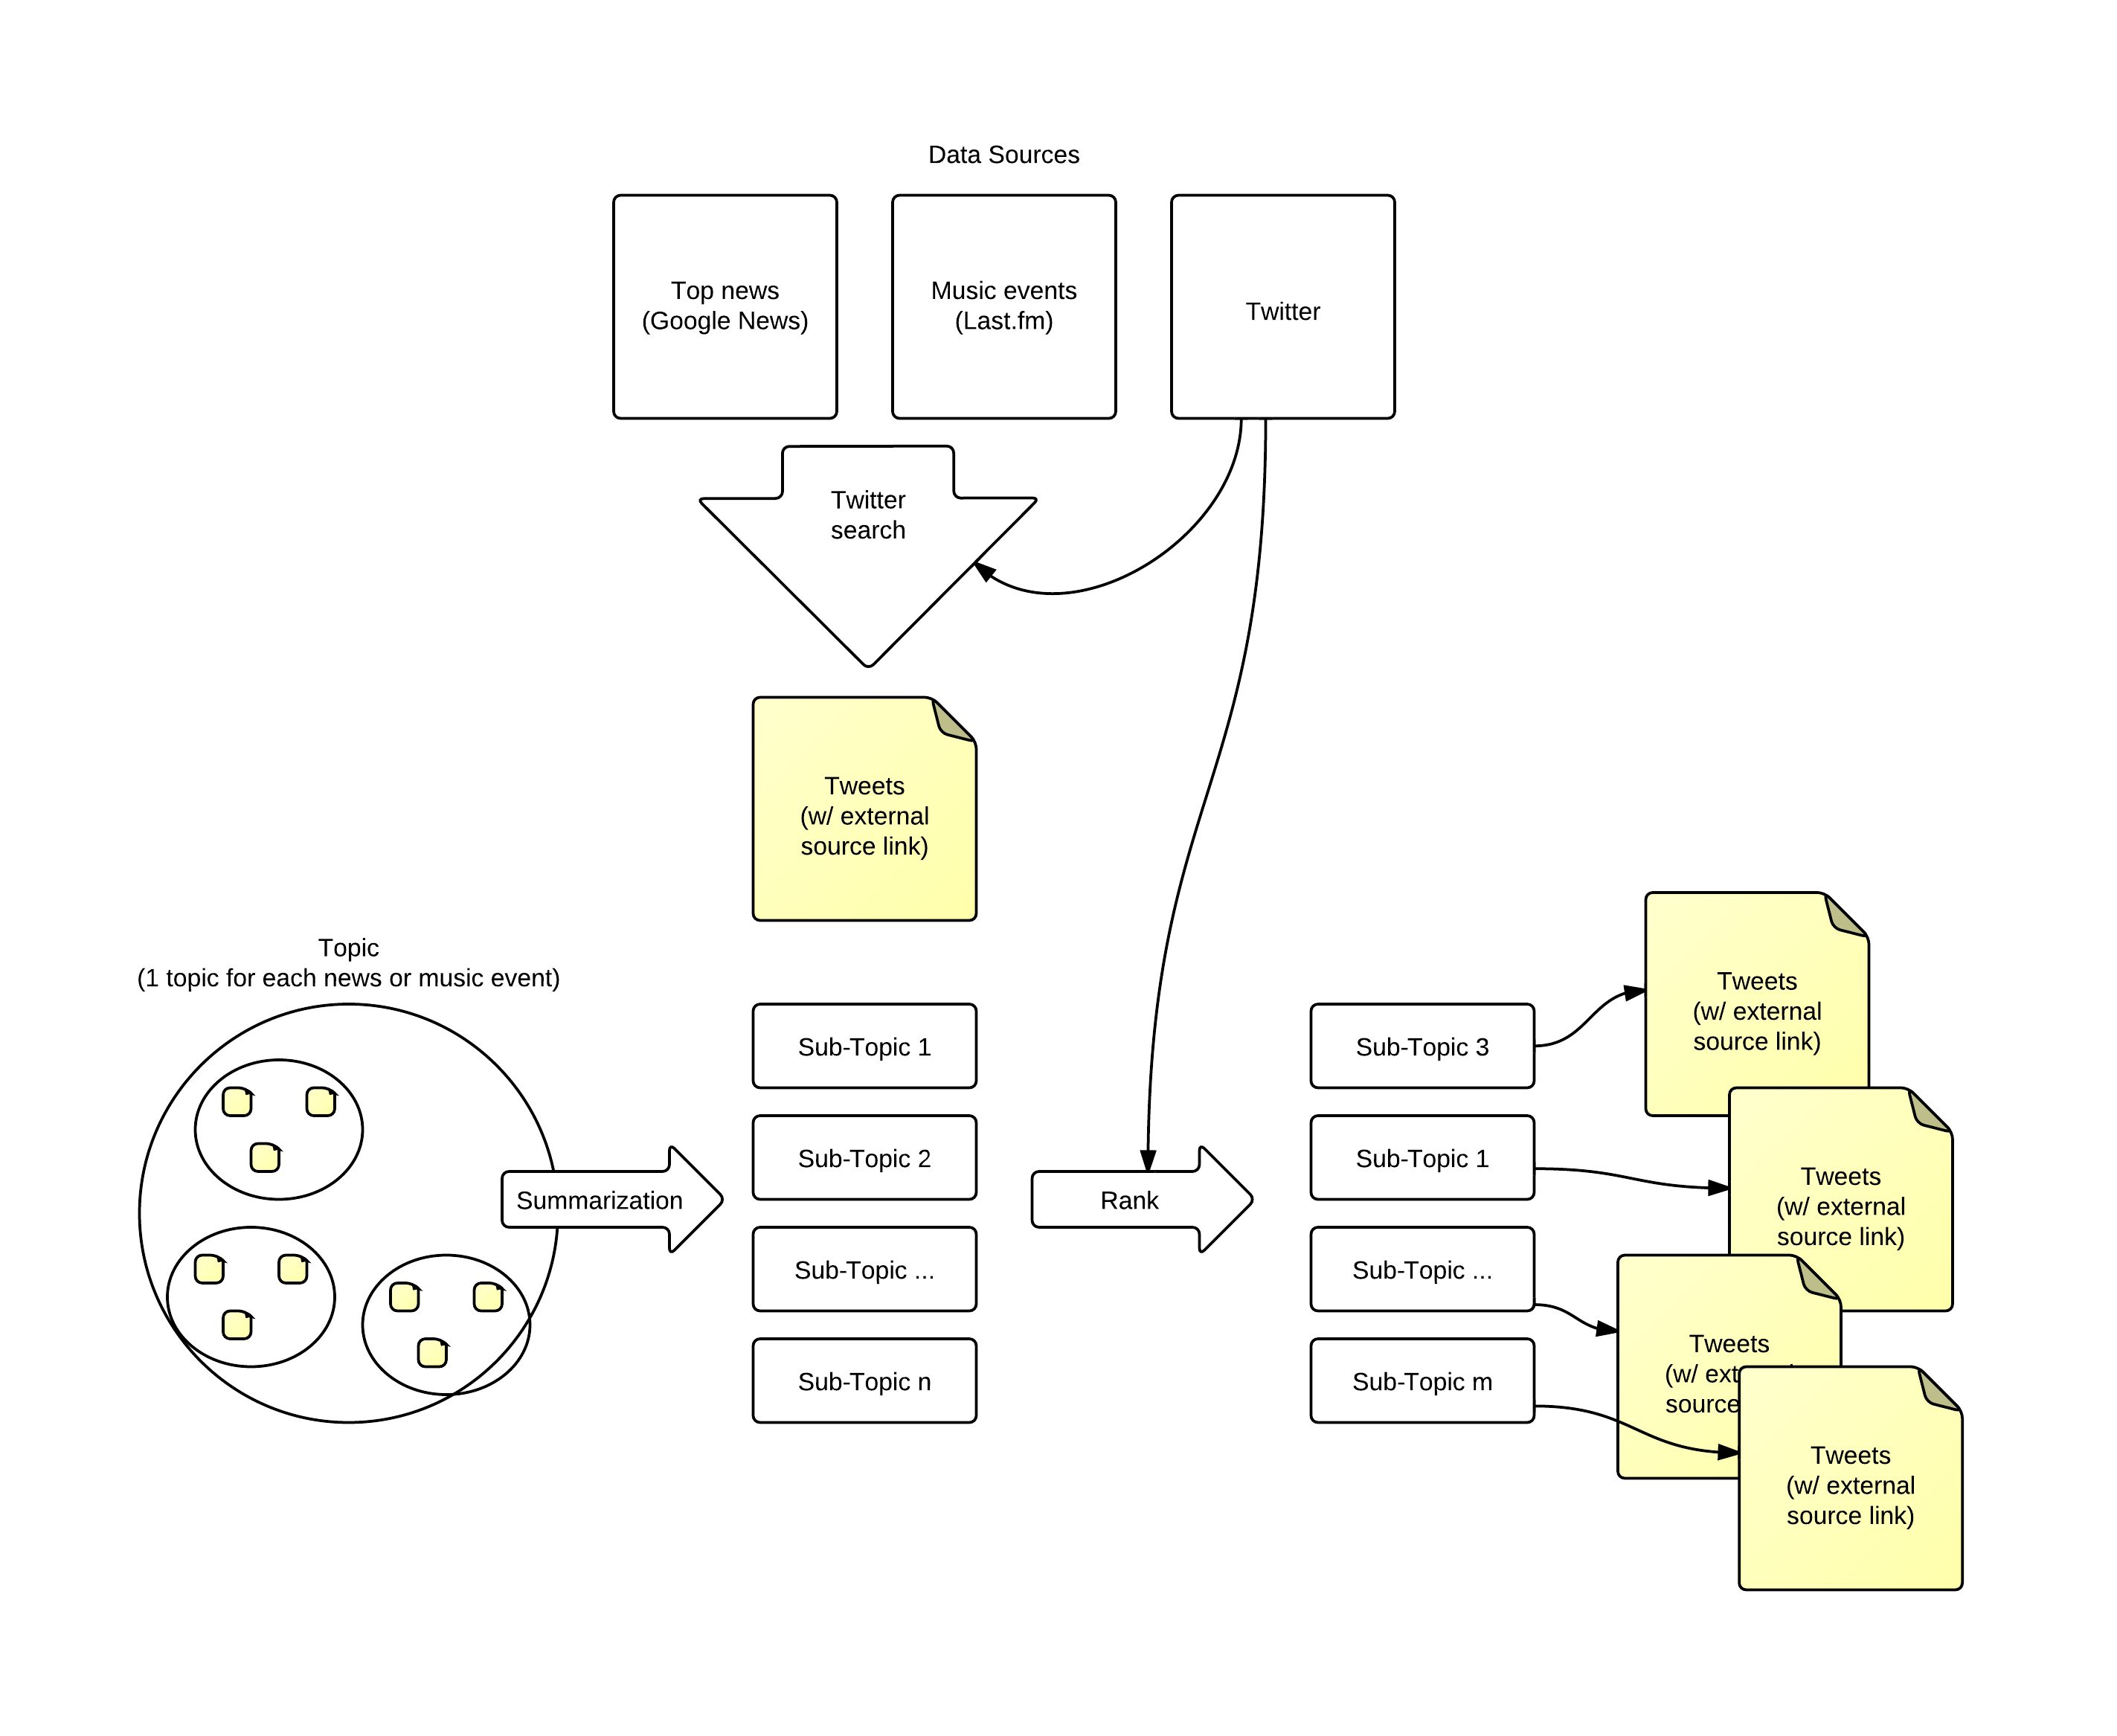
\includegraphics[width=15cm]{./img/general.png}
\caption{\label{fig:general}Diagrama general de la propuesta}
\end{figure}

  Una vez obtenidos los tweets y los documentos de cada evento, el
  sistema construirá un resumen automático de cada uno de ellos. El
  resumen consiste en una serie de sub-tópicos o temas del evento en
  cuestión. Cada tema pertenecerá a un documento en particular, y éstos
  serán los documentos que producirán el ranking a desplegar en conjunto
  con el resumen. La construcción del ranking necesitará más búsquedas
  en Twitter, ya que los indicadores para realizar las comparaciones
  dependerán tanto de los mensajes que mencionan al documento como a los
  autores de estos mensajes. Denominaremos a estos indicadores los
  \emph{Social Features} del documento.


\subsection{Social Features}
\label{sec-3.1}


   Para determinar la relevancia de los documentos incluidos en el
   resumen, se contrastarán con respecto a otros usando la información
   social que provee Twitter. Esto es, se obtendrán automáticamente
   distintos indicadores de los tweets que mencionan a estos documentos\cite{barbara},
   directa o indirectamente. Estos indicadores se presentan en el
   Cuadro \ref{tab:features}.

   \begingroup
   \fontsize{8pt}{10pt}\selectfont

\begin{longtable}{|l|l|}
\caption{\label{tab:features}Lista de Social Features a utilizar para el ranking}\\
\hline
 \textbf{Social Feature}            &  \textbf{Descripción}                                                     \\
\hline
\endhead
\hline\multicolumn{2}{r}{Continued on next page}\
\endfoot
\endlastfoot
\hline
\hline
 Tweet                              &                                                                            \\
\hline
\hline
 CONTAINS POPULAR DOMAIN TOP 100    &  Contiene una URL cuyo dominio se encuentra entre los 100 más populares    \\
 CONTAINS POPULAR DOMAIN TOP 1000   &  Contiene una URL cuyo dominio se encuentra entre los 1000 más populares   \\
 CONTAINS POPULAR DOMAIN TOP 10000  &  Contiene una URL cuyo dominio se encuentra entre los 10000 más populares  \\
 IS RETWEET                         &  Es un retweet de otro tweet: contiene `RT `                               \\
\hline
\hline
 Usuario                            &                                                                            \\
\hline
\hline
 REGISTRATION AGE                   &  Fecha de registro                                                         \\
 STATUSES COUNT                     &  Cantidad de tweets                                                        \\
 COUNT FOLLOWERS                    &  Cantidad de followers: usuarios que siguen a este usuario                 \\
 COUNT FRIENDS                      &  Cantidad de usuarios que sigue este usuario                               \\
 IS VERIFIED                        &  Si la cuenta del usuario está verificada                                  \\
 HAS URL IN PROFILE                 &  Si en la descripción del usuario hay una URL                              \\
\hline
\hline
 Tópico                             &                                                                            \\
\hline
\hline
 COUNT TWEETS                       &  Cantidad de tweets del cluster                                            \\
 AVERAGE LENGTH                     &  Largo promedio de los tweets                                              \\
 FRACTION TWEETS URL                &  Fracción de los tweets que contienen una URL                              \\
 FRACTION TWEETS MENTION            &  Fracción de los tweets que mencionan a otro usuario                       \\
 FRACTION TWEETS HASHTAG            &  Fracción de los tweets que contienen un hashtag: `\#'                     \\
 FRACTION RETWEETS                  &  Fracción de los tweets que son un retweet: contiene `RT `                 \\
 FRACTION POPULAR DOMAIN TOP 100    &  Fracción de los tweets cuya URL está entre los 100 más populares          \\
 FRACTION POPULAR DOMAIN TOP 1000   &  Fracción de los tweets cuya URL está entre los 1000 más populares         \\
 FRACTION POPULAR DOMAIN TOP 10000  &  Fracción de los tweets cuya URL está entre los 10000 más populares        \\
\hline
\end{longtable}


   \endgroup

\subsection{Prueba de concepto}
\label{sec-3.2}


   Para analizar la factibilidad del enfoque propuesto, se realizó un
   análisis preliminar de los datos publicados en Twitter. Se obtuvo
   un dataset de 2.3 millones de tweets a partir de la red 
   social, utilizando la Streaming
   API\footnote{\href{https://dev.twitter.com/docs/streaming-api}{https://dev.twitter.com/docs/streaming-api} }. De estos,
   aproximadamente 350 mil tweets incluían un enlace a otro sitio web
   en su mensaje. El siguiente desafío fue obtener las fuentes de esos
   enlaces, dado que la plataforma de Twitter utiliza un servicio de
   ``acortamiento'' de enlaces\footnote{\href{http://t.co}{http://t.co} }, por lo que el obtener
   la fuente de tales enlaces fue una tarea que tomó cierto tiempo
   comparado con el resto del análisis\footnote{Obtener los 2.3 millones de
   tweets tomó aproximadamente 22 horas, mientras que resolver las
   URLs acortadas tomó alrededor de 24 horas, a una tasa de 5 enlaces
   por segundo. }.

   En la Figura \ref{fig:dominios} se aprecia la frecuencia de enlaces con
   respecto a distintos dominios de la red.

   \begin{figure}[htb]
\centering
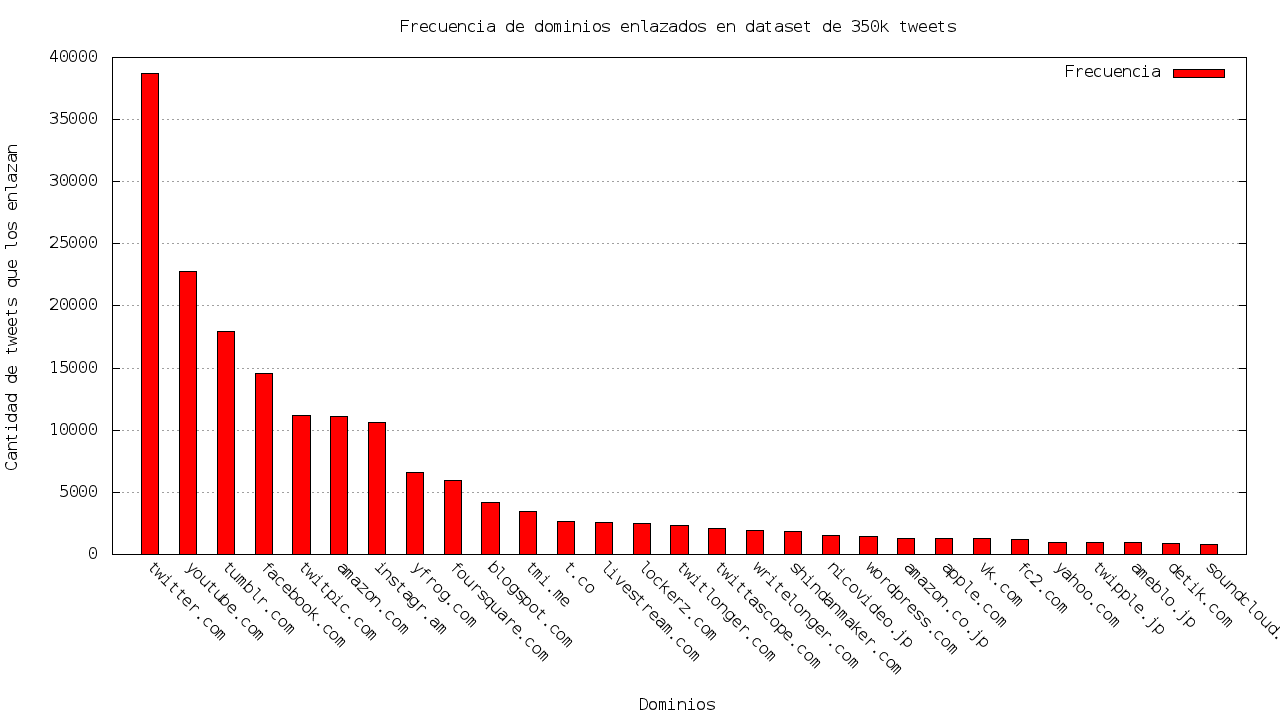
\includegraphics[width=15cm]{./img/dominios.png}
\caption{\label{fig:dominios}Histograma de frecuencia de dominios en dataset de tweets con enlaces}
\end{figure}
   
   La mayoría de los enlaces corresponden a la misma red social, lo
   que corresponde principalmente a enlaces a imágenes subidas al
   servicio de fotos y a actualizaciones de estado (enlaces que apuntan a otro
   tweet). A continuación siguen YouTube (videos), Facebook (imágenes,
   páginas, grupos, actualizaciones de estado, etc.), Tumblr
   (nueva entrada de blog), Twitpic (imágenes), Amazon (enlaces a
   productos o imágenes), Instagram (imágenes), YFrog (imágenes),
   Foursquare (check-ins en lugares físicos), Blogger (nueva entrada
   de blog, comentar un post o referenciar una imagen), etc. Una
   mención especial al servicio SoundCloud al final de la lista, cuya
   función es almacenar y compartir \emph{sonidos}.

   Dentro de la mayoría de los sitios asociados a los enlaces, se
   encuentran servicios de video, imágenes y de contenido multimedia
   (en el caso de los blogs como Tumblr, Blogspot o Wordpress).

   En la Figura \ref{fig:crecimiento} se aprecia la tasa de crecimiento de
   enlaces con respecto al tamaño del dataset obtenido hasta ese
   momento, mostrando un aumento lineal en la ocurrencia de enlaces a
   medida que crece el dataset. Según la documentación de la Streaming
   API, el método utilizado para obtener los tweets obtiene un
   \emph{muestreo} de los tweets publicados desde el momento de su
   invocación, mostrando, en caso de ser válida esa información, que
   el número de enlaces es proporcional al tamaño del dataset.

   Para el desarrollo del sistema, se utilizará otro servicio ofrecido
   por Twitter para encontrar tweets, Get
   Search\footnote{\href{https://dev.twitter.com/docs/api/1/get/search}{https://dev.twitter.com/docs/api/1/get/search} }, ya que
   el Streaming API no permite obtener tweets de momentos anteriores
   al cual es llamada. Otra ventaja de usar el otro servicio, es que
   con él es posible filtrar y obtener los enlaces no acortados por
   Twitter, lo que acelera el proceso de obtención del dataset. Para
   más detalles, véase la sección Metodología de Trabajo.

   \begin{figure}[htb]
\centering
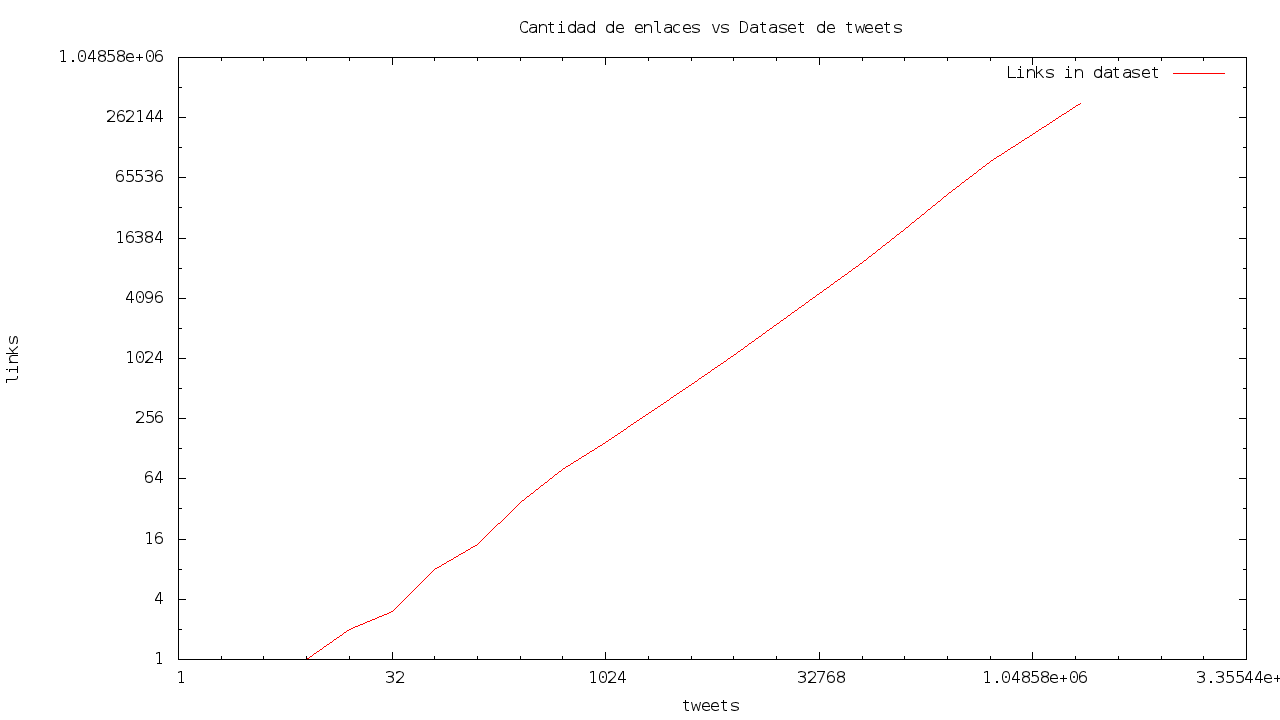
\includegraphics[width=15cm]{./img/links.png}
\caption{\label{fig:crecimiento}Gráfico log-log del crecimiento de la ocurrencia de enlaces con respecto al tamaño del dataset. Se aprecia un aumento lineal en la cantidad de enlaces con respecto al tamaño del dataset.}
\end{figure}


\pagebreak
\section{Objetivos}
\label{sec-4}

\subsection{Objetivo General}
\label{sec-4.1}

   El objetivo principal de este trabajo es lograr identificar
   contenido relevante a partir de un conjunto de documentos obtenidos
   de una o varias fuentes de datos, por medio del sistema que se
   propone implementar.

\subsection{Objetivos Específicos}
\label{sec-4.2}

\begin{itemize}
\item Comprobar la hipótesis de que es posible adaptar estrategias de
     construcción de resúmenes automáticos sobre fuentes de datos
     heterogéneas y al mismo tiempo determinar contenido multimedia
     relevante a partir de los resúmenes producidos.
\item Determinar una buena métrica para comparar la relevancia de
     distintos documentos a partir de la información obtenida de redes
     sociales online.
\item Comprobar empíricamente los resultados del sistema por medio de
     un grupo de pruebas.
\end{itemize}
\pagebreak
\section{Metodología y Plan de trabajo}
\label{sec-5}

  
\subsection{Etapas}
\label{sec-5.1}

\subsubsection{Obtención del Dataset}
\label{sec-5.1.1}

    Para obtener los eventos se utilizarán los servicios de Google
    News y Last.fm para obtener noticias y conciertos,
    respectivamente.

    Para ambos tipos de eventos se obtendrán periódicamente datos de
    éstos, y luego en Twitter se enriquecerá el dataset con tweets y
    documentos que mencionen al evento correspondiente. En el caso de
    las noticias, Google News no sólo provee la información básica de
    una noticia y una URL de alguna fuente, sino también ofrece
    noticias relacionadas (que el servicio denomina un `cluster') de
    distintas fuentes, lo cual facilitará la obtención de datos tanto
    del mismo servicio como de Twitter. Para los conciertos, por otra parte,
    el servicio de Last.fm no ofrece direcciones Web con más
    información (sino sólo datos como el título, la fecha, la ubicación y el
    grupo musical, entre otros datos de menor importancia).

    Ambos servicios mantienen una API (Application Programming
    Interface) la cual permite obtener datos en un formato de
    intercambio ligero como es el caso de JSON (JavaScript
    Object Notation). Los objetos obtenidos están garantizados de
    entregar siempre ciertos campos con datos, y para el contexto de
    este trabajo, los campos necesarios (y en común para los dos tipos
    de objetos: noticias y conciertos) son

\begin{itemize}
\item \texttt{title}, corresponde al título de la noticia o del
      concierto;
\item \texttt{content} o \texttt{description}, corresponde a una breve descripción
      del contenido de la noticia o del concierto;
\item \texttt{publishedDate} o \texttt{startDate}, la fecha de la publicación de la
      noticia y del comienzo del concierto, respectivamente y
\item \texttt{location}, \texttt{venue/location}, la ubicación del evento.
\end{itemize}
    
    Además, hay campos propios de cada tipo de evento que proveen más
    información:
    
\begin{itemize}
\item Noticias:

\begin{itemize}
\item \texttt{relatedStories}, una lista con las noticias relacionadas a la
        noticia principal, con URL, el publicador y el título de cada
        una de ellas;
\item \texttt{publisher}, la fuente que publica la noticia;
\item \texttt{clusterUrl}, la URL del ``cluster'' de la noticia: despliega
        una lista de todas las noticias relacionadas (las cuales
        pueden ser muchas). Sin embargo, la página del cluster no está
        en un formato de consumo automático, sino que es una página
        para ser vista por humanos.
\end{itemize}

\item Conciertos:

\begin{itemize}
\item \texttt{artists}, la lista de los artistas que participan en el
        concierto;
\item \texttt{attendance}, la cantidad de personas que explícitamente
        marcaron la opción de ir a ese concierto en Last.fm;
\item \texttt{tag}, una etiqueta generada por Last.fm que se sugiere
        utilizar al momento de generar contenido sobre el concierto,
        por ejemplo, al subir una foto a Flickr.
\end{itemize}

\end{itemize}
    Por otra parte, según la documentación de la API de búsqueda de
    Twitter, ésta permite obtener tweets de hasta 7 días de anticipación al
    momento de la búsqueda, y hasta 1500 tweets por búsqueda (100
    tweets en 15 páginas en un total de 15 búsquedas o llamadas a la
    API). Existe una limitación de tiempo, es decir, no es posible
    realizar más de $n$ llamadas a la API dentro de una hora. Este
    número no es publicado por Twitter, ya que según ellos, esto evita
    que se abuse del
    servicio\footnote{\href{https://dev.twitter.com/docs/rate-limiting#search}{https://dev.twitter.com/docs/rate-limiting\#search} }. Según
    la investigación realizada, es posible realizar una llamada a la
    API por segundo, dando la capacidad de 4 búsquedas completas, o
    6000 tweets por minuto en el mejor caso. 

    En el caso de la Streaming API, la cual es recomendada por Twitter
    para realizar múltiples búsquedas, la ventaja es que no tiene un
    límite de peticiones (ya que entrega un \emph{stream} de tweets,
    correspondientes a una muestra de los tweets, donde no se
    especifica cómo se seleccionan los resultados), sin embargo,
    según la prueba de concepto realizada, la cantidad de tweets es
    bastante menor en el mejor caso, además que no entrega tweets de
    días anteriores al momento en que se llama a la API. 

    Con esto en consideración, sin embargo, no existen tweets
    generados antes de una noticia que correspondan a ésta, por lo que
    utilizar la Streaming API sería ventajoso en el caso de las
    noticias; no tanto en el caso de los conciertos, pues si bien la
    cantidad de tweets mencionándolos es mayor luego de ocurrido, la
    hipótesis es que deben pasar varios días antes de disminuir
    drásticamente los tweets que los mencionan (por ejemplo, porque
    subir vídeos o fotos a la red aún es un proceso lento y tedioso,
    especialmente con los vídeos). Por lo tanto, sólo se utilizará la
    Search API.

    La metodología propuesta para obtener los eventos es la siguiente:
\begin{itemize}
\item Una vez a la semana se obtendrán las noticias más importantes
      del día\footnote{Por ejemplo, esta URL retorna las noticias más
      relevantes en la edición en inglés de Google News:
      \href{https://ajax.googleapis.com/ajax/services/search/news?v=1.0&topic=h}{https://ajax.googleapis.com/ajax/services/search/news?v=1.0\&topic=h} },
      y luego se buscará en Twitter los tweets que mencionen a esas
      noticias.
\item Una sola vez se obtendrán los conciertos de distintos lugares
      del mundo: Estados Unidos, Brasil, Alemania y Chile.
\item Cada día se harán búsquedas de tweets de las noticias
      almacenadas.
\item Dentro de una ventana de tiempo de 7 días, se buscarán los
      tweets que mencionen a cada concierto.
\item De cada documento que sea mencionado en los tweets (de la forma
      de URLs), se obtendrá su contenido en texto y se almacenará.
\end{itemize}
\subsubsection{Construcción de Resúmenes}
\label{sec-5.1.2}

    Una vez obtenido algún evento con sus tweets y documentos
    asociados, se utilizará un algoritmo de construcción de resúmenes
    automáticos sobre el evento normalizado. La normalización del
    evento consiste en construir un vector de documentos y palabras, y
    se utilizará el algoritmo \textsc{SummHMM} definido en
    \cite{events}.

    Con el resumen construido, cada cluster correspondiente a un
    sub-tópico de éste corresponderá a su vez a un documento del
    dataset inicial, el cual puede también abarcar contenido
    multimedia el cual será contrastado con los demás clusters del
    resumen para generar un orden.

\subsubsection{Ranking y presentación de resultados}
\label{sec-5.1.3}

    
    Con cada clustering correspondiente a un tópico o evento, la
    siguiente fase consiste en tomar los documentos representativos de
    cada cluster del tópico y generar un orden mediante una
    ponderación de sus \emph{social features} descritos en la descripción de
    la propuesta. Con esto se medirá la importancia de un documento con
    respecto a la popularidad, relevancia y reputación de éste.

    Finalmente, los documentos seleccionados serán presentados en una
    interfaz (web) en este orden de importancia, ya sea para ser
    consumido por humanos como por máquinas (por ejemplo, en algún formato
    como \texttt{JSON}).

\subsection{Herramientas a utilizar}
\label{sec-5.2}

   Para el desarrollo del sistema se utilizarán distintas herramientas
   tanto para obtener datos de las fuentes determinadas anteriormente
   como para generar los resúmenes, crear el ranking y presentar los
   resultados.

   Se utilizará el lenguaje \texttt{Python} \footnote{\href{http://www.python.org/}{http://www.python.org/} },
   dada la experiencia previa, la flexibilidad del lenguaje para
   realizar prototipos rápidos y la gran cantidad de librerías
   existentes para manipular datos y conectarse a distintos
   servicios. En particular: 

\begin{itemize}
\item \texttt{Twython} \footnote{\href{https://github.com/ryanmcgrath/twython}{https://github.com/ryanmcgrath/twython} }, una
     librería para realizar búsquedas y acceder fácilmente a la
     información que provee Twitter. Con esta librería se realizaron
     algunas búsquedas para probar la factibilidad de la metodología
     de obtención de datos descrita en esta sección.
\item Para acceder a distintos sitios web para obtener documentos, la
     librería \texttt{mechanize}
     \footnote{\href{http://wwwsearch.sourceforge.net/mechanize/}{http://wwwsearch.sourceforge.net/mechanize/} } emula un Web
     Browser en \texttt{python}, y para analizar y procesar las páginas HTML
     de cada sitio, \texttt{BeautifulSoup}
     \footnote{\href{http://www.crummy.com/software/BeautifulSoup/}{http://www.crummy.com/software/BeautifulSoup/} } cumple tal
     objetivo. Para almacenar y empaquetar datos, \texttt{simplejson}
     \footnote{\href{https://github.com/simplejson/simplejson}{https://github.com/simplejson/simplejson} } permite el manejo
     de JSON de manera flexible y rápida.
\end{itemize}
   Para el almacenamiento de los datos, se consideró utilizar una base
   de datos relacional como \texttt{MySQL}, sin embargo, en pos de la
   flexibilidad, para no crear y modificar un modelo de datos
   relacional cuando haya que realizar cambios a éste, se decidió
   utilizar un sistema de datos \emph{schemaless} (sin esquema, o también
   conocido como \emph{NoSQL}). Se han considerado \texttt{MongoDB}
   \footnote{\href{http://www.mongodb.org/}{http://www.mongodb.org/} } y \texttt{Redis} \footnote{\href{http://redis.io/}{http://redis.io/} } para
   este propósito, con las respectivas librerías en \texttt{python} que se
   encargan de crear una interfaz entre el lenguaje de programación y
   el software de base de datos.

   La librería de minería de datos \texttt{Orange}
   \footnote{\href{http://orange.biolab.si/}{http://orange.biolab.si/} } ofrece varias funcionalidades como
   Clasificación, Clustering, Reglas de Asociación, entre otras. No se
   ha visto en detalle las capacidades y utilidad de esta herramienta,
   pero queda en consideración su uso en el futuro.

   Para la presentación de los datos, se tiene en consideración
   utilizar un framework web para crear una aplicación web que
   despliegue los resultados obtenidos. Entre las posibilidades,
   \texttt{Django} \footnote{\href{https://www.djangoproject.com/}{https://www.djangoproject.com/} } y \texttt{Flask}
   \footnote{\href{http://flask.pocoo.org/}{http://flask.pocoo.org/} } son buenas alternativas.

   Para versionar y mantener los cambios del código del sistema a
   implementar, se utilizará el sistema de control de versiones \texttt{Git}
   \footnote{\href{http://git-scm.com/}{http://git-scm.com/} } y el servicio
   GitHub\footnote{\href{http://www.github.com/}{http://www.github.com/} } para almacenarlo
   remotamente. Tanto el trabajo adelantado hasta la fecha y este
   mismo informe están en este
   servicio\footnote{\href{https://github.com/mquezadav/cc6909}{https://github.com/mquezadav/cc6909} }.  

   Para el desarrollo de este informe y los siguientes, se utilizó y
   utilizará \texttt{GNU Emacs} \footnote{\href{http://www.gnu.org/software/emacs/}{http://www.gnu.org/software/emacs/} } y su
   extensión \texttt{org-mode} \footnote{\href{http://orgmode.org/}{http://orgmode.org/} } que 
   permite escribir documentos rápidamente y generar el archivo $\LaTeX$
   (y correspondientemente, PDF) equivalente.

\pagebreak
\section{Plan de Trabajo}
\label{sec-6}

  En el Cuadro \ref{tab:plan} se aprecia el plan de trabajo propuesto
  para el desarrollo. Se considera el desarrollo de dos prototipos
  incrementales (\texttt{P1} y \texttt{P2}) que consideren la retroalimentación y el ajuste
  de parámetros y algoritmos que sea necesario realizar, dentro del
  contexto de 17 semanas de trabajo.
  
  \begingroup
  \fontsize{8pt}{10pt}\selectfont

  \newcommand{\x}{\checkmark}
   
\begin{longtable}{|l||l|l|l|l|l|l|l|l|l|l|l|l|l|l|l|l|l|}
\caption{\label{tab:plan}Plan de trabajo}\\
\hline
 Módulo / Semana                  &  1   &  2   &  3   &  4   &  5   &  6   &  7   &  8   &  9   &  10  &  11  &  12  &  13  &  14  &  15  &  16  &  17 \\
\hline
\endhead
\hline\multicolumn{18}{r}{Continued on next page}\
\endfoot
\endlastfoot
\hline
 Obtención del dataset            &  \x  &  \x  &  \x  &  \x  &  \x  &  \x  &  \x  &  \x  &  \x  &  \x  &  \x  &  \x  &  \x  &      &      &      &      \\
 Construcción de resúmenes (P1)   &  \x  &  \x  &  \x  &  \x  &      &      &      &      &      &      &      &      &      &      &      &      &      \\
 Construcción de resúmenes (P2)   &      &      &      &      &  \x  &  \x  &  \x  &  \x  &      &      &      &      &      &      &      &      &      \\
 Ranking (P1)                     &      &      &  \x  &  \x  &  \x  &  \x  &      &      &      &      &      &      &      &      &      &      &      \\
 Ranking (P2)                     &      &      &      &      &      &      &  \x  &  \x  &  \x  &  \x  &      &      &      &      &      &      &      \\
 Presentación de resultados       &      &      &      &      &      &      &      &      &      &      &  \x  &  \x  &  \x  &      &      &      &      \\
 Redacción de informe de memoria  &      &      &      &      &      &      &      &      &      &      &  \x  &  \x  &  \x  &  \x  &  \x  &  \x  &  \x  \\
\hline
\end{longtable}

   
   \endgroup

   


\pagebreak


\begin{thebibliography}{9}
\bibitem{concerts} 

Hila Becker, Dan Iter, Mor Naaman, Luis Gravano. \emph{Identifying Content for Planned Events Across Social Media Sites}. WSDM'12.

\bibitem{events}

Deepayan Chakrabarti, Kunal Punera. \emph{Event Summarization using Tweets}. AAAI 2011.

\bibitem{clusterers}

Hila Becker, Mor Naaman, Luis Gravano. \emph{Learning Similarity Metrics for Event Identification in Social Media}. WSDM'10.

\bibitem{selecting}

Hila Becker, Mor Naaman, Luis Gravano. \emph{Selecting Quality Twitter Content for Events}. AAAI 2011.

\bibitem{real}

Hila Becker, Mor Naaman, Luis Gravano. \emph{Beyond Trending Topics: Real-World Event Identification on Twitter}. AAAI 2011.

\bibitem{barbara}

Castillo, C., Mendoza, M., Poblete, B.: \emph{Information Credibility on Twitter}. In The World Wide Web Conference (WWW), Hyderabad, India. 2011.

\bibitem{survey}

Das, D.. and Martins, A.: \emph{A survey on automatic text
summarization}. Language Technologies Institute, Carnegie Mellon
University. 2007.

\bibitem{microblogs}

Sharifi, B.; Hutton, M.-A.; and Kalita, J. 2010. \emph{Summarizing
     microblogs automatically}. In HLT.

\bibitem{earthquakes}

Sakaki, T.; Okazaki, M.; and Matsuo, Y. \emph{Earthquake shakes
twitter users: Real-time event detection by social sensors}. In WWW 2010.

\end{thebibliography}





































\end{document}
